\documentclass[11pt,a4paper]{article}
\usepackage[utf8]{inputenc}
\usepackage{graphicx}
\usepackage{tikz}
\usepackage{pgfplots}
\pgfplotsset{compat=1.13}

\title{Iterative Closest Point \\ {\large Computer Vision 2 - Assignment 1}}
\author{Ysbrand Galama \\ 10262067 \and David van Erkelens \\ 10264019}
\date{\today}

\begin{document}
\maketitle

\section{Introduction}

\section{Results}
\begin{figure}
\centering
\includegraphics[width=.49\textwidth,height=.49\textwidth]{graphs/sam_i.png}
\includegraphics[width=.49\textwidth,height=.49\textwidth]{graphs/sam_o.png}
\caption{The point clouds of the sample data in 3D space (left) and the transformed pair with an error of $0.000947$ after $30$ iterations of the ICP algorithm (right).}
\label{fig:sam0}
\end{figure}

\begin{figure}
\centering
\input{graphs/graph1.tex}
\caption{Accuracy and amount of iterations (with a maximum of 15) after ICP on the sample data, using: all points, uniform sampling with step-size $2$,$17$,$47$ and $91$, random sampling with $p=0.8$,$p=0.5$,$p=0.1$ and $p=0.01$, and random sampling with $p=0.8$,$p=0.5$,$p=0.1$ and $p=0.01$ after each iteration.}
\label{fig:sam1}
\end{figure}

\begin{figure}
\centering
\centerline{
\begin{tikzpicture}
%\end{axis}
\begin{axis}[
    width=1\textwidth,
    height=.22\textheight,
    ymin=0,ymax=17,
   % xmin=0,xmax=21,
    xtick={0,...,15},
    xticklabels={},
    %x tick label style={color=white},
	ylabel={Iterations},
	axis y line*=left,
	enlargelimits=0.05,
	legend style={at={(0.5,-0.4)},
	anchor=north,legend columns=-1},
	ylabel near ticks,
	ybar,
	%ymajorgrids=true,
	%xmajorgrids=false,
    grid style=dashed
]
%\addlegendimage{blue, mark=*}
%\addlegendimage{only marks, orange!80, mark=square*}
%\addlegendimage{only marks, purple!70, mark=square*}
%\legend{Accuracy, Train time, Test time}
\addplot[color=orange!80,fill=orange!80]
	coordinates {
	(0,7) (2,15) (3,6) (4,3) (5,2) (7,8) (8,15) (9,15) (10,15) (12,12) (13,15) (14,15) (15,15)
    };
\end{axis}
\begin{semilogyaxis}[
%\begin{axis}[
    title={Iterations and accuracy of different sub-sampeling settings},
    width=\textwidth,
    height=.22\textheight,
    ymin=0.0001, ymax=1,
    %xmin=0,xmax=21,
	xtick={0,...,15},
	xticklabels={
		%linear,poly:d=2,poly:d=3,poly:d=4,poly:d=5,poly:d=6,poly:d=7,poly:d=8,poly:d=9,rbf:$\gamma$=0.0,rbf:$\gamma$=0.1,rbf:$\gamma$=0.2,rbf:$\gamma$=0.3,rbf:$\gamma$=0.4,rbf:$\gamma$=0.5,rbf:$\gamma$=0.6,rbf:$\gamma$=0.7,rbf:$\gamma$=0.8,rbf:$\gamma$=0.9,rbf:$\gamma$=1.0,
		all,$\,$,$sample_{2}$,$sample_{17}$,$sample_{47}$,$sample_{91}$,$\,$,$rand1_{0.8}$,$rand1_{0.5}$,$rand1_{0.1}$,$rand1_{0.01}$,$\,$,$randi_{0.8}$,$randi_{0.5}$,$randi_{0.1}$,$randi_{0.01}$,
	},
	x tick label style={rotate=30, anchor=north east, inner sep=0mm},
	%xlabel={\hspace{1cm}${\underbrace{\text{\hspace{5cm}}}\atop\text{polynomial}}$\hspace{0.4cm}${\underbrace{\text{\hspace{7cm}}}\atop\text{rbf}}$},
	%xlabel style={at={(0.5,-0.03)}},
	ylabel=Mean Squared Error,
	axis y line*=right,
	enlargelimits=0.05,
	legend style={at={(0.5,-0.4)},
	anchor=north,legend columns=-1},
	%ybar stacked,
	ylabel near ticks
]
\addplot[mark=*,blue,jump mark mid]
	coordinates {
	(-1,1000) (0,0.0018) (1,1000) (2,0.0028) (3,0.0011) (4,0.0012) (5,0.0013) (6,1000) (7,0.0020) (8,0.0023) (9,0.0115) (10,0.0998) (11,1000) (12,0.016) (13,0.0056) (14,0.0244) (15,0.1368) (16,1000)
    };
\end{semilogyaxis}
\end{tikzpicture}
}
\caption{Accuracy and amount of iterations (with a maximum of 15) after ICP on the sample data with Gaussian noise of $\mu=0.01$, using: all points, uniform sampling with step-size $2$,$17$,$47$ and $91$, random sampling with $p=0.8$,$p=0.5$,$p=0.1$ and $p=0.01$, and random sampling with $p=0.8$,$p=0.5$,$p=0.1$ and $p=0.01$ after each iteration.}
\label{fig:sam2}
\end{figure}

\begin{figure}
\centering
\input{graphs/graph2.tex}
\caption{Accuracy and amount of iterations (with a maximum of 15) after ICP on the sample data with Gaussian noise of $\mu=0.1$, using: all points, uniform sampling with step-size $2$,$17$,$47$ and $91$, random sampling with $p=0.8$,$p=0.5$,$p=0.1$ and $p=0.01$, and random sampling with $p=0.8$,$p=0.5$,$p=0.1$ and $p=0.01$ after each iteration.}
\label{fig:sam3}
\end{figure}

\begin{figure}
\centering
\begin{tabular}{cc}
\includegraphics[width=.49\textwidth,height=.49\textwidth]{graphs/tot1.png} &
\includegraphics[width=.49\textwidth,height=.49\textwidth]{graphs/tot2.png} \\ (a) & (b) \\
\includegraphics[width=.49\textwidth,height=.49\textwidth]{graphs/tot4.png} &
\includegraphics[width=.49\textwidth,height=.49\textwidth]{graphs/tot10.png} \\ (c) & (d)
\end{tabular}
\caption{The point cloud of the model after ICP moddeling every frame (a), every second frame (b), every fourth frame (c) and every tenth frame (d) with the frame before.}
\label{fig:}
\end{figure}

\section{Discussion}

\end{document}